\documentclass{article}
\usepackage[utf8]{inputenc}
\usepackage{hyperref}
\usepackage{listings}
\usepackage{xcolor}

\definecolor{codegreen}{rgb}{0,0.6,0}
\definecolor{codegray}{rgb}{0.5,0.5,0.5}
\definecolor{codepurple}{rgb}{0.58,0,0.82}
\definecolor{backcolour}{rgb}{0.95,0.95,0.92}

\lstdefinestyle{mystyle}{
    backgroundcolor=\color{backcolour},   
    commentstyle=\color{codegreen},
    keywordstyle=\color{magenta},
    numberstyle=\tiny\color{codegray},
    stringstyle=\color{codepurple},
    basicstyle=\ttfamily\footnotesize,
    breakatwhitespace=false,         
    breaklines=true,                 
    captionpos=b,                    
    keepspaces=true,                 
    numbers=left,                    
    numbersep=5pt,                  
    showspaces=false,                
    showstringspaces=false,
    showtabs=false,                  
    tabsize=2
}

\lstset{style=mystyle}
\hypersetup{
    colorlinks=true,
    linkcolor=blue,
    filecolor=magenta,      
    urlcolor=cyan,
    pdftitle={Overleaf Example},
    pdfpagemode=FullScreen,
    }

\author{Tarushii Goel}
\date{2020}

\usepackage[letterpaper, margin=1in]{geometry}
\usepackage{natbib}
\usepackage{graphicx}
\usepackage{amsmath}



\begin{document}

\begin{center}
\fbox{\fbox{\parbox{5.5in}{\centering
Problem Set: Pytorch \\
Due date:  9/29/19\\
Total Points: 15\\
If you run out of room for an answer, use scratch paper and staple it to this sheet.}}}
\end{center}
 
\vspace{5mm}
 
\makebox[\textwidth]{Name and Grade:\enspace\hrulefill}
 
\vspace{5mm}

\begin{enumerate}
	\item (10 points) Using what you learned about Pytorch in the lecture, as well as your own exploration of the torch.nn and torch.optim modules, write a program that classifies objects in the CIFAR-10 dataset. You will find that you can tackle this problem, which is much harder than fitting the sine curve, in only a few lines of extra code. Attach a copy of your code as well as a short reflection. Guiding Questions: What did you learn about Pytorch through this exercise? What architecture did you use? What was your accuracy? What steps did you take to increase the accuracy? How long did you need to train? Did you perform and image preprocessing or data augmentation, and if you did, how did that affect accuracies? \\ 
	You will want to use these lines to access the dataset:
	\begin{lstlisting}
	from torchvision import datasets
	cifar10 = datasets.CIFAR10(root='data/', train=True, download=True)
	cifar10_val = datasets.CIFAR10(root='data/', train=False, download=True) \end{lstlisting}
	\pagebreak
	\item (5 points) Replicate these two CNN architectures and train them on the CIFAR-10 Dataset (you may need to change input/output layer dimensions, do this as you like). How do the accuracies compare? Why do you think that is? You can attach your code for this as well. 
\begin{center}
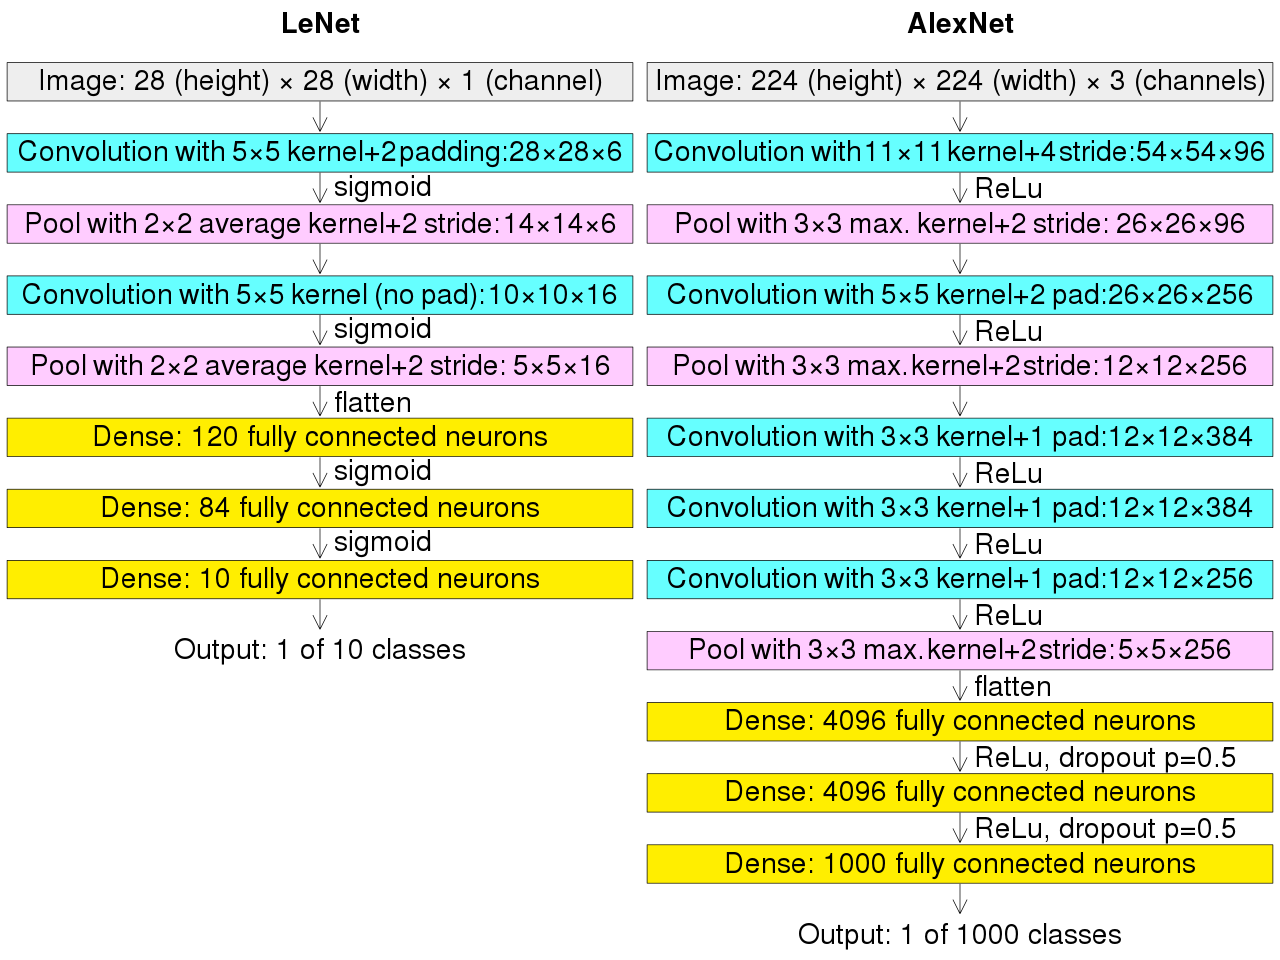
\includegraphics[scale=0.3]{networks.svg}
\end{center}

\end {enumerate}
\end{document}
